\newpage

\section{Ruby-on-Rails}
\label{sec:rails}
\epigraph{Ruby on Rails is a breakthrough in lowering the barriers of entry to programming. Powerful web applications that formerly might have taken weeks or months to develop can be produced in a matter of days.}{Tim O'Reilly, Gründer von O'Reilly Media}


Für das Projekt IT-jobs-und-stellen.de soll das Webframework Ruby-on-Rails\index{Ruby-on-Rails} verwendet werden. Rails wurde 2004 von der Firma 37signals\footnote{\url{http://37signals.com/}} unter der Leitung von David Heinemeier Hansson entwickelt und erlangte seitdem eine wachsende Popularität. Rails inspirierte viele andere Frameworks, wie z.B. cakePHP, Symfony, Groovy on Grails und ASP.NET MVC\footnote{\url{http://de.wikipedia.org/wiki/Ruby_On_Rails\#Verwandte_Frameworks}}.
% \footnote{ Sowie weitere PHP-Frameworks -- \url{http://www.h3rald.com/articles/rails-inspired-php-frameworks/}}

\bordergraphic{material/rails.png}
Viele professionelle Websites, die meist als Startup begannen, setzen bis heute auf Rails\index{Ruby-on-Rails}. Darunter Github, eine sehr beliebte Community für OpenSource-Programmierer, Groupon, das führenden Unternehmen bei Online-Gutscheinen, XING, eine deutsche Online\hyp{}Community für Business-Kontakte, aber auch nicht-StartUps, z.B. Yellow Pages, die Gelben Seiten der USA \citep{ruby_on_rails_2011}. Viele bekannte Firmen nutzen Rails auch auf die eine oder andere Weise, z.B. zur Entwicklung ihrer internen Webanwendungen. Dazu gehören BBC, Cisco, IBM, Oracle, die NASA, Siemens oder Yahoo\footnote{Weitere Firmen: \url{http://www.workingwithrails.com/high-profile-organisations}}.

Im Folgenden werden die Grundprinzipien und -konzepte von Ruby-on-Rails\index{Ruby-on-Rails} näher erläutert.

\subsection{Konzepte von Rails}
\label{sec:railsconcepts}
Rails\index{Ruby-on-Rails} ist ein Applikationsframework für Webanwendungen und basiert auf dem \glossar{MVC} \glossar{patterns}, welches eine 3-Schichten-Architektur darstellt. Jede Schicht hat fest definierte Aufgaben und alle Schichten bilden bei Rails normalerweise zusammen ein Dreigespann, \textbf{Ressource} genannt. Im Folgenden werden die Schichten kurz erläutert und am Beispiel einer Ressource "`Job"' erklärt.
\begin{description}
 \item[Model] In Klassen dieser Schicht werden Zugriffe auf die Persistenzschicht vorgenommen. Meist geschieht dies durch Ausführung von SQL-Befehlen auf eine relationale Datenbank\index{Datenbank}. Innerhalb von Rails\index{Ruby-on-Rails} ist das Schreiben von SQL aber meist nicht notwendig, da das \glossar{ORM}-\textit{ActiveRecord\index{ActiveRecord}} häufig verwendete SQL-Befehle abstrahiert. Die Geschäftslogik soll per Definition zu großem Teil in dieser Schicht erfolgen.

 Für einen Job ist das ein Modell\index{Ruby-on-Rails!Modell}, welches die Datenbank\index{Datenbank}tabelle "`jobs"' anspricht und z.B. die Attribute "`titel"', "`datum"' und "`beschreibung"' besitzt. Dabei können auf diesem Level auch datenbankunabhängige Constraints, die \textbf{Validierung\index{Ruby-on-Rails!Validierung}en}, definiert werden, z.B. dass ein Job nur dann gespeichert werden soll, wenn der Titel mindestens 20 Zeichen lang ist und das Datum mindestens das Heutige ist.
 \item[Controller\index{Ruby-on-Rails!Controller}] Klassen dieser Schicht beinhalten Methoden, die von außen per HTTP erreichbar sind. Diese Methoden kommunizieren mit den korrespondierenden Models und bestimmen, welche View\index{Ruby-on-Rails!View} im Einzelnen ausgeliefert wird. Weitere Funktionen eines Controllers sind Authentifizierung und Autorisierung\footnote{Authentifizierung: Wer ist der Nutzer?\\Autorisierung: Was darf der Nutzer?}.\\
 Standardmäßig stellt Rails\index{Ruby-on-Rails} die \glossar{CRUD}-Operationen bereit, welche in Form eines REST-Schemas angesprochen werden (mehr zu REST später).
%  \footnote{Representational State Transfer die HTTP-Methoden GET, POST, PUT, DELETE werden in Kombination mit einem definierten URL-Schema direkt auf die Aktionen \texttt{Auflisten, Anzeigen, Bearbeiten, Löschen, neu anlegen} gemappt.
%  \url{http://en.wikipedia.org/wiki/Representational_State_Transfer}}
 \item[View\index{Ruby-on-Rails!View}] Eine View ist in der Regel ein Stück HTML-Code, welches einem Model zugeordnet ist, das dem Clienten bei einer bestimmten Aktion ausgeliefert wird. Neben HTML ist auch JavaScript\index{JavaScript} oder XML eine mögliche Auslieferungsform.\\
 Für den Job wären Beispiele für eine View\index{Ruby-on-Rails!View} die Auflistung aller Jobs, einen Job im Detail anzeigen sowie das Formular zum Anlegen und Bearbeiten eines Jobs.
\end{description}
% TODO Graphik konkretisieren auf /jobs/12
 \begin{figure}[h]
  \centering
  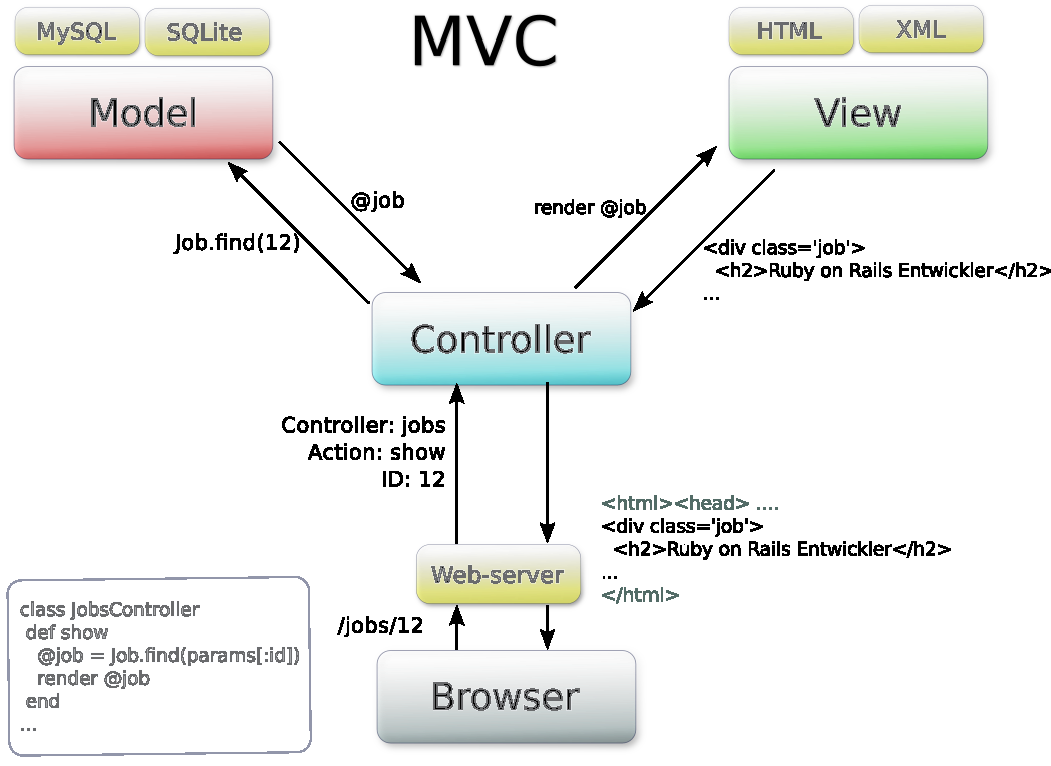
\includegraphics[width=0.7\textwidth]{./diagrams/mvc.pdf}
  % mvc-rails.png: 500x472 pixel, 72dpi, 17.64x16.65 cm, bb=
  % SOURCE
  \caption{MVC-Modell von Rails am Beispiel einer Anfrage /jobs/12}
  \label{fig:mvcrails}
\end{figure}
In Abbildung \ref{fig:mvcrails} ist der Ablauf einer Anfrage an den Server dargestellt. Die Anfrage des Browsers an die Website \texttt{http://localhost/jobs/12} wird über den Webserver, z.B. Apache2, an die Railsanwendung gestellt. Innerhalb von Rails wird dieser Anforderungsstring anhand der Routen, die die Anwendung anbietet, gematcht. In unserem Falle würde \texttt{/jobs/12} auf den Controller\index{Ruby-on-Rails!Controller} \texttt{Jobs} aufgelöst werden. Innerhalb dieses Controllers wird eine Methode (Aktion) \texttt{show} erwartet.
Diese Methode wird nun ihrerseits eine Anfrage an das Model Job stellen, den Job mit der ID 12 aus der Datenbank\index{Datenbank} zu holen. Danach wird ein HTML-Template zur Detailanzeige des Jobs generiert.


Neben diesem architektonischen Konzept verfolgt Rails\index{Ruby-on-Rails} noch andere Strategien, um das Entwickeln produktiver zu gestalten.
\begin{description}
 \item[Convention over Configuration] Rails wurde konzipiert, um als Framework komplett out-of-the-box zu funktionieren. Außer der Datenbank\index{Datenbank}einstellung wird im Vorfeld keine Konfiguration benötigt. Diese Methodologie zieht sich auch durch das Ökosystem von Ruby\index{Ruby}. Die meisten externen Bibliotheken, bei Ruby \glossarpl{gem}\index{Gem} genannt, erschließen sich und funktionieren bereits binnen weniger Minuten. Dies macht das prototypische Entwickeln äußert effektiv. Weiterhin ist die Struktur eines Railsprojektes fest definiert. So gibt es u. a. einen Ordner \texttt{app} mit den Model-, Controller\index{Ruby-on-Rails!Controller}- und View\index{Ruby-on-Rails!View}-Dateien und einen Ordner \texttt{test}, der wiederum in \texttt{unit}, \texttt{functional}, \texttt{integration} und \texttt{performance} unterteilt ist. So finden sich Railsprogrammierer auch in fremden Projekten sofort zurecht.
 \item[Don't repeat yourself (DRY)] Hier ist das Ziel, die Duplikation so weit wie möglich zu reduzieren, um bei Änderungen nur an einer Stelle ansetzen zu müssen. Ein Beispiel ist die Definition der Attribute der Objekte durch das \glossar{ORM}. Im Gegensatz zu anderen ORM-Frameworks ist dies bei Rails\index{Ruby-on-Rails} nicht notwendig. Rails erstellt automatisch Getter und Setter für die in der Datenbank\index{Datenbank} definierten Tabellenspalten. Hintergrund ist, dass die Definition über Name und Typ der Attribute bereits in der Datenbank vorliegt und eine Wiederholung im Quellcode dem DRY-Prinzip widerspräche.
 \item[REST] Representational State Transfer ist eine Software-Architektur für HTTP-Web\hyp{}Services. Dabei werden neben den Standard-HTTP-Methoden GET und POST auch die selten benutzen Verben DELETE und PUT verwendet, um Aktionen auf eine Ressource zu definieren. Das Ziel ist ein sehr einfaches Design der URLs.

 Eine Verwendung der \glossar{CRUD}-Operationen mittels Rails\index{Ruby-on-Rails} würde am Beispiel einer Ressource \texttt{jobs} wie folgt aussehen:
  \begin{description}
  \item[GET /jobs.html] Auflisten aller Jobs, Ausgabe als HTML Format.
  \item[GET /jobs/12.xml] Job mit der ID 12 anzeigen, Formatiere als XML.
  \item[POST /jobs] Einen Job anlegen. Alle benötigten Parameter wie Titel, Beschreibung oder Datum sollten im POST-Body der HTTP-Anfrage enthalten sein.
  \item[PUT /jobs/12] Den Job mit der ID 12 aktualisieren. Die Eigenschaften, die aktualisiert werden, müssen als Parameter mit übergeben werden.
  \item[DELETE /jobs/12] Lösche den Job mit der ID 12.
  \end{description}
 Rails macht das Arbeiten im Kontext dieser Architektur sehr einfach und REST gilt als die bevorzugte Methode in der Community APIs\footnote{Application Programming Interface --  Eine Schnittstelle, um extern mit der Anwendung zu kommunizieren} zu erstellen.
 \item[Codegeneratoren] Rails bietet viele Codegeneratoren an, um schnell benötigte Klassen, Testfälle und Datenbanktabellen anzulegen.  Wie mit Hilfe der Codegeneratoren praktisch gearbeitet wird, wird später in Kapitel 7 dargelegt werden.
 \item[Full-Stack-Webframework] Rails\index{Ruby-on-Rails} \borderquote{Rails will have strong defaults. They might change over time but Rails will remain opinionated.}{D. Hansson, Begründer von Rails}
bringt out-of-the-box alles mit, was zur Webentwicklung benötigt wird. Im Gegensatz zu anderen Webframeworks wurde für Datenbankanbindung\index{Datenbank}, Templatesystem, JavaScript-Framework\index{JavaScript}, Testframework und Webserver-API bereits eine Vorauswahl getroffen. Im aktuellen Rails 3.1 sind dies ActiveRecord\index{ActiveRecord} (Datenbank-Framework), ERB (Templating-Sprache), JQuery (JavaScript-Framework) sowie Test/Unit\index{Test/Unit-Framework} und Rack (Kommunikationsinterface für Komponenten). Die meisten dieser Komponenten lassen sich zwar leicht austauschen, Rails selbst aber behauptet "`opinionated"', also rechthaberisch / eigensinnig, zu sein und dem Entwickler Standards vorzugeben \citep{david_heinemeier_hansson_railsconf_2011}.

\end{description}

Eine komplette Einführung in die Programmierung mit Rails\index{Ruby-on-Rails} soll nicht Bestandteil dieser Diplomarbeit sein. Für eine weitere Einarbeitung seien die folgende Quellen empfohlen:
\begin{description}
 \item[Rails for Zombies] Dies ist ein moderner, interaktiver Onlinekurs. Greg Pollack und das Team von RailsEnvy verpackt die Lektionen in humorvolle, interaktive Lernerfahrungen. Jeweils eingeleitet durch ein Video, muss der Teilnehmer Aufgaben direkt im Quelltext lösen. Die Teilnahme ist kostenlos.\\
 \url{http://railsforzombies.org/}
 \item[Agile Webdevelopment with Ruby-on-Rails] Das quasi-Standardwerk, u. a. geschrieben vom Rails-Begründer David Hansson. Das Buch wird meist parallel mit einer neuen Rails-Version in einer neuen Auflage gedruckt, aktuell die dritte \citep{ruby_agile_2009}.
 \item[Rails Guides] Die von Ruby-on-Rails herausgegebenen "`Rails Guides"' sind eine gut strukturierte, kostenlose Online-Dokumentation, die nahezu alle Aspekte von Rails beleuchtet und anhand von praktischen Beispielen erläutert.\\
 \url{http://guides.rubyonrails.org/getting_started.html}
 \end{description}



\subsection{Diskussion}
Nach einem kurzen Überblick über Rails\index{Ruby-on-Rails} sollen nun die Eigenschaften des Frameworks sowie die sich daraus ergebenden Auswirkungen auf das Testen diskutiert werden.

\paragraph{Nachteile}

Oft wird angeführt,\randbem{Performanz} dass Ruby\index{Ruby} als Skriptsprache und Rails\index{Ruby-on-Rails} als darauf aufbauendes Framework eine schlechte Performanz besitzt und dadurch ungeeignet für große Webanwendungen ist.\\
Anderseits existieren Erfahrungen, dass eine clevere Architektur und Caching für skalierende Anwendung entscheidender ist als die letztendliche Ausführungszeit \citep{kirk_haines_ruby_2010}.
Dass eine Skalierung mit Rails\index{Ruby-on-Rails} möglich ist, zeigen z.B. Groupon, der führende Online-Coupon-Anbieter mit mehr als 50 Mio. Abonnenten und Twitter, die jeweils Rails verwenden bzw. verwendet haben \citep{ruby_on_rails_2011}.
%http://www.socialshopping.com/Groupon/news/Groupon-hits-50m-Subscribers-Shopping-site-sensation-201101210398/

Da Rails\index{Ruby-on-Rails} ein komplettes Webframework ist,\randbem{Auswahl der Komponenten} wurden bei der Auswahl der einzelnen Komponenten bereits Entscheidungen getroffen.  Erst Anfang 2011 gab es dazu Kritik aus Teilen der Community, da ab der Version 3.1 \textit{CoffeeScript} und \textit{SASS} Bestandteile einer Rails-Distribution sind \citep{peter_cooper_rails_2011}. Beide sind Zwischensprachen, die in JavaScript\index{JavaScript}, respektive CSS kompilieren und diese um Funktionalität erweitern. Allerdings kann jeder selbst wählen, ob er diese verwenden möchte.


Interaktion mit Legacy-Software ist nicht immer möglich. \randbem{Integration in bestehende Software}ActiveRecord\index{ActiveRecord} reserviert einige Spaltennamen wie \texttt{type} und \texttt{class}. Eine Benennung der Spalten sollte der Ruby\index{Ruby}-Namenskonvention entsprechen, also nur Buchstaben, Zahlen und Unterstriche enthalten. Ansonsten können die Spalten nur über Umwege angesprochen werden. Rails\index{Ruby-on-Rails} ist äußerst effektiv, wenn man den gegebenen Konventionen folgt. Im Umkehrschluss bedeutet dies, dass man deutlich ineffektiver wird, wenn man die Konventionen von Rails ignoriert, z.B. wegen äußerer Umstände und Anforderungen.\\
Rails\index{Ruby-on-Rails} verzichtet auf die Verwendung von Constraints innerhalb der Datenbank\index{Datenbank}. In einigen Fällen, z.B. Bankensoftware, sind diese aber unbedingt erforderlich.

Ein Nachteil aus Sicht des Projektmanagement ist der Mangel\randbem{Mangel an Entwicklern} an freien Ruby-on-Rails\index{Ruby-on-Rails} Programmierern auf dem Arbeitsmarkt\footnote{z.B. \url{http://rubypays.blogspot.com/2011/04/rubyruby-on-rails-development-job.html}}. So kann bei einem langfristig angesetzten Projekt u. U. die Wartung nicht garantiert werden.

\paragraph{Vorteile}
Rails\index{Ruby-on-Rails} unterstützt den Software-Lebenszyklus,\randbem{Software\hyp{}Lebenszyklus} indem es von Haus aus drei Umgebungen definiert: Development, Test und Production. Diese unterscheiden sich in der Datenbank\index{Datenbank}, die sie benutzen, und Konfigurationsparametern zu Caching und Performanz. Weitere Umgebungen (z.B. Staging) können jederzeit definiert werden.


Dank der Modularität können als Persistenzgrundlage sowohl \randbem{Flexible Datenanbindung}relationale Datenbank\index{Datenbank}en wie MySQL, SQlite und Oracle, aber auch andere Formen wie NoSQL-Datenbanken transparent verwendet werden. Dank einer einfach zu verstehenden Syntax ist das Schreiben von SQL in vielen Fällen überflüssig und die Sicherheitslücke einer SQL-Injection wird ausgeschlossen. Bei relationalen Datenbanken verwendet ActiveRecord\index{ActiveRecord} standardmäßig Transaktionen, sofern die Datenbank dies unterstützt.



Rails\index{Ruby-on-Rails} bietet eine gute Ausgangsbasis, um sichere Websoftware zu entwickeln.\randbem{Sicherheit} Das Verwenden eines Datenbank\index{Datenbank}frameworks macht SQL-Injections unmöglich. \\
Cross-Site-Request-Forgery und Session-Angriffe werden erschwert, da Session- und Cookie-Variablen standardmäßig verschlüsselt werden und bei Nutzung der Formulargeneratoren ein CSRF-Token generiert wird, um Replay-Angriffe zu unterbinden.

\borderquote{I needed to be way more productive...}{D. Hansson}
Die Codegeneratoren, die Aufteilung in \glossar{MVC} und die mitgelieferten Werkzeuge machen Rails\index{Ruby-on-Rails} äußerst produktiv und in wenigen Minuten lassen sich so bereits erste Anwendungen bauen. Der Begründer von Rails führte z.B. in einer Konferenz vor, wie man mit Rails ein Blog in 15 Minuten bauen kann\footnote{http://media.rubyonrails.org/video/rubyonrails.mov}.


\paragraph{Testen mit Rails}
Rails\index{Ruby-on-Rails} bietet ausgezeichnete Voraussetzungen zum Softwaretest. Dafür spricht, dass...

\begin{itemize}
  \item benötigte Bibliotheken bereits mitgeliefert werden. Dies umfasst einen Test-Runner, vorkonfigurierte Test-Datenbanken (auf Basis von SQLite) und das Testframework Test/Unit,
  \item die Verwendung stark erleichtert wird, da Rails\index{Ruby-on-Rails} beim Nutzen der Codegeneratoren analoge Testdateien gleich mitgeneriert,
 \item neben den mitgelieferten Tools das Rails\index{Ruby-on-Rails}-Ökosystem eine Vielzahl von Testtools bereitstellt, u.a. Rspec (\glossar{BDD}-Testframework), Rcov (Testabdeckung\index{Test!Testabdeckung}), diverse Mock\index{Test-Double!Mock}bibliotheken (mocha, FlexMock, RR, Rspec Mocks), Tools zum Generieren und Bereitstellen von Testdaten\index{Test!Testdaten} (Fixtures, Factories, Faker) und \glossarpl{metrik}\index{Code-Metrik} (metric-fu).
 \item das Testen einen sehr hohen Stellenwert in der Ruby- und Rails-Comumnity hat. Nahezu alle namhaften Ruby-Programmierer schreiben umfassende Tests \citep{devries_rails_2008}. Das Resultat ist, dass auch fast alle \glossarpl{gem}\index{Gem} bei Ruby eine "`solid suite of tests"' haben \citep{devries_rails_2008}.
\end{itemize}

Rails\index{Ruby-on-Rails} unterstützt verschiedene Testarten out-of-the-box:
\begin{description}
 \item[Unittest\index{Test!Unittest}s] oder Modell\index{Ruby-on-Rails!Modell}tests (model test)\\
 Testziel: alle (komplexeren) Methoden, die das Modell\index{Ruby-on-Rails!Modell} anbietet, seine Validierung\index{Ruby-on-Rails!Validierung}en und Beziehungen zu anderen Objekten.
 \item[Funktionale Tests] Untersuchungsgegenstand sind die Controller\index{Ruby-on-Rails!Controller}. \\
 Testziel: Getestet wird meist der Arbeitsablauf innerhalb eines Controller\index{Ruby-on-Rails!Controller}s, also Weiterleitungen, Benachrichtigungen und welches Template gerendert wird.
 Damit können gleichzeitig auch View\index{Ruby-on-Rails!View}-Tests unternommen werden, also z.B. die Untersuchung, ob ein bestimmtes HTML-Element auf der Webseite zu sehen ist.
 \item[Integrationstests] Es wird ein Browser simuliert, der von außen auf die Applikation zugreift.\\
 Zielstellung: Testen komplexer Interaktionen zwischen verschiedenen Teilen der Software.\\
 Beispiel: Ein User loggt sich ein und legt einen neuen Job an.
 \item[Performanz-Tests] Eine Testart, die alle Methoden aus Unittest\index{Test!Unittest}s und funktionalen Tests beinhaltet.\\
 Zielstellung: Lokalisation von Performanz-Flaschenhälsen auf allen Bereichen der Software. \\
 Beispiel: Es werden 1000 Jobs generiert und geprüft, ob die Anzeige schnell genug läuft.
\end{description}
